\subsection{Dashboard Module}
Το Dashboard είναι το κεντρικό Module της εφαρμογής, που φαίνεται και στην αρχική σελίδα και εμφανίζει μέσο του MIDashboard Component 4 διαφορετικά κομμάτια. Το πρώτο κομμάτι είναι η μπάρα αναζήτησης, το δεύτερο κομμάτι είναι ένας παγκόσμιος χάρτης, το τρίτο κομμάτι είναι στα δεξιά του χάρτη και αποτελείται απο γραφήματα και συγκεντρωτικά στοιχεία και το τέταρτο και τελευταίο κομμάτι είναι τα κύρια δεδομένα της εφαρμογής όπως ο πιο δημοφιλής ηθοποιός, η ή ταινία με τα μεγαλύτερα έσοδα κ.λ.π όπως φαίνεται στο σχήμα \ref{wire:dashboard}.

\begin{figure}[H]
  \centering
  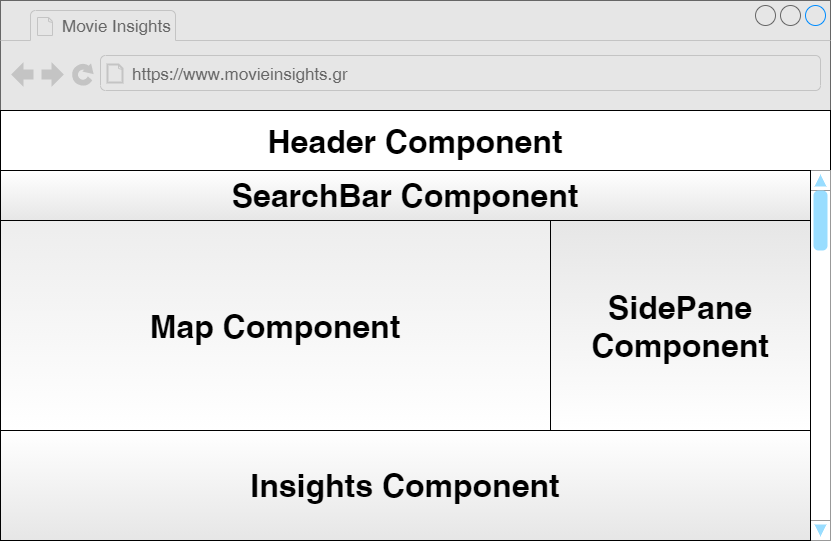
\includegraphics[width=145mm]{Chapters/5 - Architecture/Client/Images/dashboard_struct.png}
  \caption{Βασική διάταξη Web εφαρμογής}
  \label{wire:dashboard}
\end{figure}

Το Dashboard Module δεν ορίζει δίκο του router παρά μόνο ένα Route /app/* και ενα Redirect απο το κεντρικό Route / στο /app το οποίο είναι η κεντρική σελίδα καθώς δεν χρειάζεται κάτι σύνθετο. 

Ο τρόπος που λειτουργεί είναι ο εξής. Είναι επιλεγμένη για παράδειγμα μια κατηγορία "Στοιχεία για την χώρα Ελλάδα".
Σε αυτήν την κατηγορία στα δεδομένα υπάρχουν οι πιο δημοφιλείς ηθοποιοί, παραγωγοί, σκηνοθέτες, συγγραφείς που έχουν συμμετάσχει σε ταινίες που είτε η παρήγαγε η Ελλάδα είτε η Ελλάδα ήταν χώρα συμπαραγωγής. Αναφέρει επίσης την πιο δημοφιλή εταιρία παραγωγής που συνεργάστηκε η Ελλάδα αλλά και την πιο δημοφιλή χώρα συμπαραγωγής και είδος ταινίας. Επιπρόσθετα αναφέρει τα μέσα και συνολικά έσοδα/έξοδα καθώς και το καθαρό κέρδος. Όλα αυτά τα στοιχεία υπάρχουν επίσης και ανά χρόνο, για όσα χρόνια υπάρχουν στην βάση δεδομένων για την Ελλάδα. Όλες οι κατηγορίες λειτουργούν με τον ίδιο τρόπο με την εξαίρεση της κατηγορίας ανά άτομο. Που εκεί εκτός από την επιλογή χρόνου, υπάρχει και η επιλογή ρόλου, με διαθέσιμους ρόλους: ηθοποιός, σκηνοθέτης, συγγραφέας και παραγωγός. Για τα άτομα υπάρχουν συγκεντρωτικά στοιχεία μόνο ανά ρόλο και όχι συνολικά, καθώς είναι διαφορετικά τα δεδομένα. Πάραυτα όλα τα στοιχεία ανά ρόλο υπάρχουν και ανά χρόνο.

Το Dashboard Module περιέχει μόνο ένα Component το ΜΙDashboard Component. Όλα τα δεδομένα που υπολογίζονται μέσα απο το Dashboard Module στέλνονται απευθείας στο ΜΙDashboard Component.

Μέσω των Component που δηλώνονται και δομείται όλη η εφαρμογή καθιστάται εφικτή η πλοήγηση σε όλο το εύρος των δεδομένων της εφαρμογής. Ενώ θα μπορούσε σε κάθε Component, που επιρεάζει τα δεδομένα που εμφανίζονται, να υλοποιηθεί η λογική της αλλαγής των δεδομένων, προτιμήθηκε όλα αυτα τα Component απλα να αλλάζουν την διεύθυνση στην γραμμή διεύθυνσης του browser και με βάση την διεύθυνση που άλλαξε χωρίς να γίνεται ανακατεύθυνση το Dashboard Module καταλαβαίνει τι χρειάζεται να αλλάξει, αλλάζει τα δεδομένα μέσω του Redux State Manager, και ύστερα στέλνει τα δεδομένα σε όλα τα επιμέρους Components για να αλλάξουν. Ένω ακούγεται πιο σύνθετη τεχνική, χρησιμοποιήθηκε για την ευκολία διαχείρισης και συντήρησης του κώδικα, καθώς στην άλλη περίπτωση θα έπρεπε σε περίπτωση αλλαγής του κώδικα εμφάνισης των δεδομένων, σε κάθε Component που άλλαζε δεδομένα. Ενώ με αυτήν την υλοποίηση τα πάντα βρίσκονται σε ένα μέρος. Ένας ακόμα σημαντικός λόγος που προτιμήθηκε η συγκεκριμένη τεχνική είναι η προσβασιμότητα στα δεδομένα αυτά. Λόγω της φύσης της αρχιτεκτονικής της εφαρμογής και όντας SPA, υπάρχει ουσιαστικά μόνο μια σελίδα που είναι πρόσβασιμη απο εναν Browser. Αυτή ειναι η index.html. Ένα αρχείο HTML με όλο τον κώδικα της εφαρμογής. Χωρίς την αλλαγή της διεύθυνσης, ένας χρήστης θα έπρεπε να μπει στην αρχική σελίδα και να εκτελέσει κάποιες ενέργειες έτσι ώστε να φτάσει στο ίδιο σημείο που βρισκόταν πριν. Με την αλλαγή της διεύθυνσης όμως, οχι μόνο μπορεί να επανέλθει στο σημείο στο οποίο βρισκόταν αλλά μπορεί και να μοιραστεί τον σύνδεσμο με κάποιον άλλον χρήστη και να κοιτάνε τα ίδια δεδομένα. 

Το Dashboard Module λοιπόν παρακολουθεί τις αλλαγές διευθύνσεων που γίνονται μετα την βασική διεύθυνση /app/ και με την χρήση κάποιον βοηθητικών συναρτήσεων αλλάζει τα δεδομένα όπως φαίνεται στον κώδικα \ref{code:urlIntercept}.

\begin{figure}[h]
    \begin{TypeScriptcode}
handleViewChange = () => {
    const path = this.props.location.pathname;
    if (this.state.path !== path || !this.state.pathHandled) {
      if (!this.state.pathHandled) {
        let pathMatch: match;
        if ((pathMatch = matchPath(path, "/app/:entity(country|company|genre)/:id-:name/:year(\\d{4})?"))) {
          this.handleGenericChange(pathMatch.params['entity'], +pathMatch.params['id'], +pathMatch.params['year']);
        } else if ((pathMatch = matchPath(path, "/app/person/:id-:name/:role([A-z]+)?/:year(\\d{4})?"))) {
          this.handlePersonChange(+pathMatch.params['id'], +pathMatch.params['year'], pathMatch.params['role']);
        } else if ((pathMatch = matchPath(path, "/app/:general(general)?/:year(\\d{4})?"))) {
          this.handleGeneralChange(+pathMatch.params['year']);
        }
        this.scrollElement();
        if (this.state.path !== path)
          this.setState({path});
      }
      if (this.state.path !== path) {
        this.setState({pathHandled: false});
      }
    }
}
    \end{TypeScriptcode}
    \caption{Αλγόριθμος παρακολούθησης αλλαγής στην γραμμή διευθύνσεων ενός Browser.}
   \label{code:urlIntercept}
\end{figure}

Η αλλαγή της διεύθυνσης στην γραμμή διευθύνσεων του Browser, δημιουργείται απο μια βοηθητική συνάρτηση όπως φάινεται στον κώδικα \ref{code:urlBuilder}. Με αυτόν τον τρόπο όλα τα Components που έχουν ως σκοπό την αλλαγή των δεδομένων μπορούν να αλλάξουν εύκολα την διεύθυνση χρησιμοποιώντας αυτήν την συνάρτηση, και αν αλλάξει ποτέ η δομή της διεύθυνσης η αλλαγή θα γίνει μόνο μέσα σε αυτήν την συνάρτηση διευκολύνοντας παράλληλα την συντήρηση και την αντιμετώπιση προβλημάτων του κώδικα.

\begin{figure}[h]
    \begin{TypeScriptcode}
function |$\textbf{generateNavigationLink}$|(entity?: BaseNamedEntity, role?: CreditRole, year?: number, entityType?: EntityType) {
  let type = undefined;
  if (entity) {
    if (entityType) {
      type = entityType.toLowerCase();
    } else if (isMovie(entity)) {
      type = 'movie';
    } else if (isPerson(entity)) {
      type = 'person';
    } else if (isCompany(entity)) {
      type = 'company';
    } else if (isCountry(entity)) {
      type = 'country';
    } else if (isGenre(entity)) {
      type = 'genre';
    }
  } else if (year) {
    type = 'general';
  }
  return `/app${type ? `/${type}` : ''}${entity ? `/${entity.id}-${normalizeText(entity.name)}` : ''}${role && type === 'person' ? `/${role}` : ''}${year ? `/${year}` : ''}`;
}
    \end{TypeScriptcode}
    \caption{Αλγόριθμος δημιουργίας διεύθυνσης αλλαγής δεδομένων.}
   \label{code:urlBuilder}
\end{figure}

Το Redux State Manager χρησιμοποιήθηκε για 2 λόγους. Προσφέρει μια εύκολη διεπαφή που βασίζεται στο Immutability των δεδομένων συμβάλλοντας δραστικά στην μείωση των Side Effects, αλλα επίσης χρησιμοποιήθηκε σαν ένα Facade για την απόκτηση των δεδομένων απο την υπηρεσία.

Γνωρίζοντάς ότι οποιαδήποτε ενέργεια εμπεριέχει κάποιου είδους επικοινωνία με μια εξωτερική υπηρεσία αυξάνει σημαντικά τον χρόνο της διεκπεραίωσης της, και έχοντας σαν δεδομένο οτι η JavaScript που τρέχει μέσα σε έναν Browser τρέχει σε ένα και μοναδικό νήμα (Thread), η εμπειρία του χρήστη θα ήταν πολύ άσχημη όταν θα ζητούσε νέα δεδομένα απο τον Server, καθώς η Web Εφαρμογή θα ήταν μη αποκρίσιμη για αρκετό διάστημα μέχρι την απόκτηση των δεδομένων και την εμφάνιση τους. Για αυτόν τον λόγο χρησιμοποιήθηκε ένα πρόσθετο στο Redux Fraemwork, που επιτρέπει την ασύγχρονη απόκτηση δεδομένων και την αποθήκευση τους στο κεντρικό State της εφαρμογής. Όλα τα Components που εξαρτιούνται απο αυτό το Global State, όταν αλλάξει θα αλλάξουν και αυτά τα δεδομένα που εμφανίζουν.

Όπως προαναφέρθηκε το Dashboard Component περιέχει 4 σημαντικά Component που εμφανίζουν όλα τα απαραίτητα δεδομένα.

\subsubsection{SearchBar Component}
Το πρώτο Component μέσα στο MIDashboard Component είναι η γραμμή αναζήτησης, MISearchBar Component. Το MISearchBar Component δεν προσφέρει την δυνατότητα γενικής αναζήτησης αλλά μόνο την δυνατότητα επιλογής ενός αποτελέσματος απο τις προτάσεις της μηχανής αναζήτησης. Οι προτάσεις δημιουργούνται απο την μηχανή αναζήτησης μέσο του Server όπως προαναφέρθηκε νωρίτερα κάθε φορά που ο χρήστης γράφει οποιοδήποτε γράμμα στην μπάρα αναζήτησης όπως φαίνεται στον κώδικα \ref{code:searchbar_suggestion}.

\begin{figure}[H]
    \begin{TypeScriptcode}
async function getSuggestions(value: string): Promise<ACResult[]> {
    const results: AutoComplete = (await Service.search(value)).data;
    return results._
      .map(result => {
        result.e.forEach(e => {
          e.i = result.i
        })
        return result;
      })
      .filter(result => result.e.length > 0);
}
    \end{TypeScriptcode}
    \caption{Αλγόριθμος ανάκτησης προτάσεων αποτελεσμάτων μηχανής αναζήτησης}
   \label{code:searchbar_suggestion}
\end{figure}

Οι προτάσεις της μηχανής αναζήτησης εμφανίζονται με μια μικρή εικόνα στα αριστερά και το κείμενο του αποτελέσματος ακριβώς από διπλά. Ανάλογα με το κείμενο της αναζήτησης που έγραψε ο χρήστης προσπαθεί να υπογραμμίσει με μπλε χρώμα τα γράμματα που βρέθηκαν στα αποτελέσματα όπως φαίνεται στην εικόνα \ref{layout:misearchbar}.
\begin{figure}[H]
  \centering
  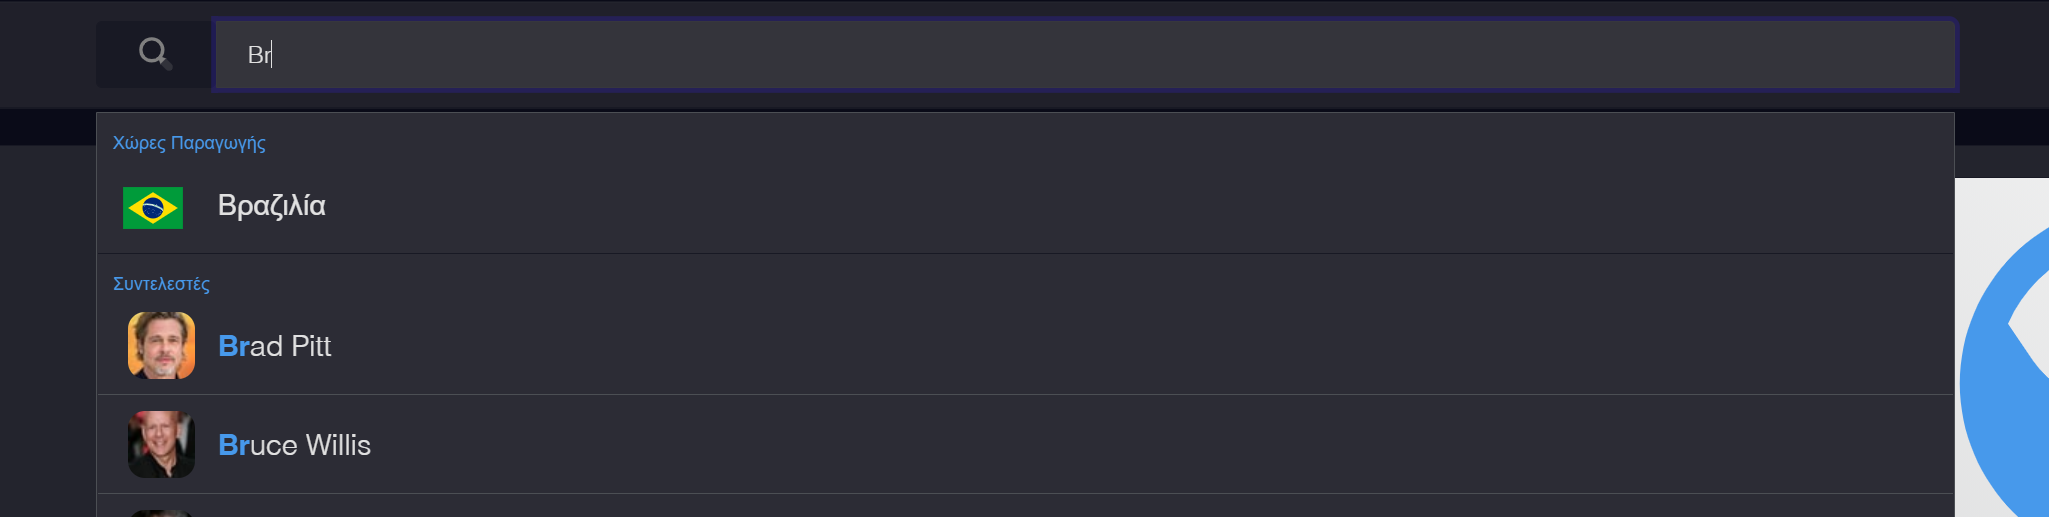
\includegraphics[width=145mm]{Chapters/5 - Architecture/Client/Images/misearchbar_results.png}
  \caption{MISearchBar Component}
  \label{layout:misearchbar}
\end{figure}
Οταν επιλεγεί ενα απο τα προτεινόμενα αποτελέσματα η μπάρα αναζήτησης σβήνει και αλλάζει η διεύθυνση όπως φαίνεται στον κώδικα \ref{code:searchbar_urlchange}

\begin{figure}[H]
    \begin{TypeScriptcode}
private onSearch = (val: ACEntity) => {
  this.props.history.push(AppUtils.|\textbf{generateNavigationLink}|(val, null, null, val.i));
}
    \end{TypeScriptcode}
    \caption{Αλγόριθμος αλλαγής διεύθυνσης απο το MISearchBar Component}
   \label{code:searchbar_urlchange}
\end{figure}

\subsubsection{MapComponent}
Το δεύτερο είναι το Map Component και είναι ένα Component το οποίο προσφέρει ένα προ-ρυθμισμένο Chart από την βιβλιοθήκη Highcharts Highmaps και προσφέρει μια εύκολη διεπαφή για την αλληλεπίδραση και εμφάνιση δεδομένων σε αυτόν τον χάρτη όπως φαίνεται στο σχήμα \ref{layout:mapcomponent}. Κάθε φορά που ο δείκτης του ποντικιού περνάει πάνω απο μια χώρα εμφανίζεται ενα tooltip που γράφει το όνομα της χώρας και σε πόσες ταινίες έχει συμμετάσχει αυτή η χώρα. Όταν πατηθεί μια χώρα θα επιλεγεί εκτός αν ήταν ήδη επιλεγμένη που τότε θα σταματήσει να είναι επιλεγμένη και θα αλλάξει η διεύθυνση όπως φαίνεται στον κώδικα στο σχήμα \ref{code:map_urlchanger}.
\begin{figure}[H]
  \centering
  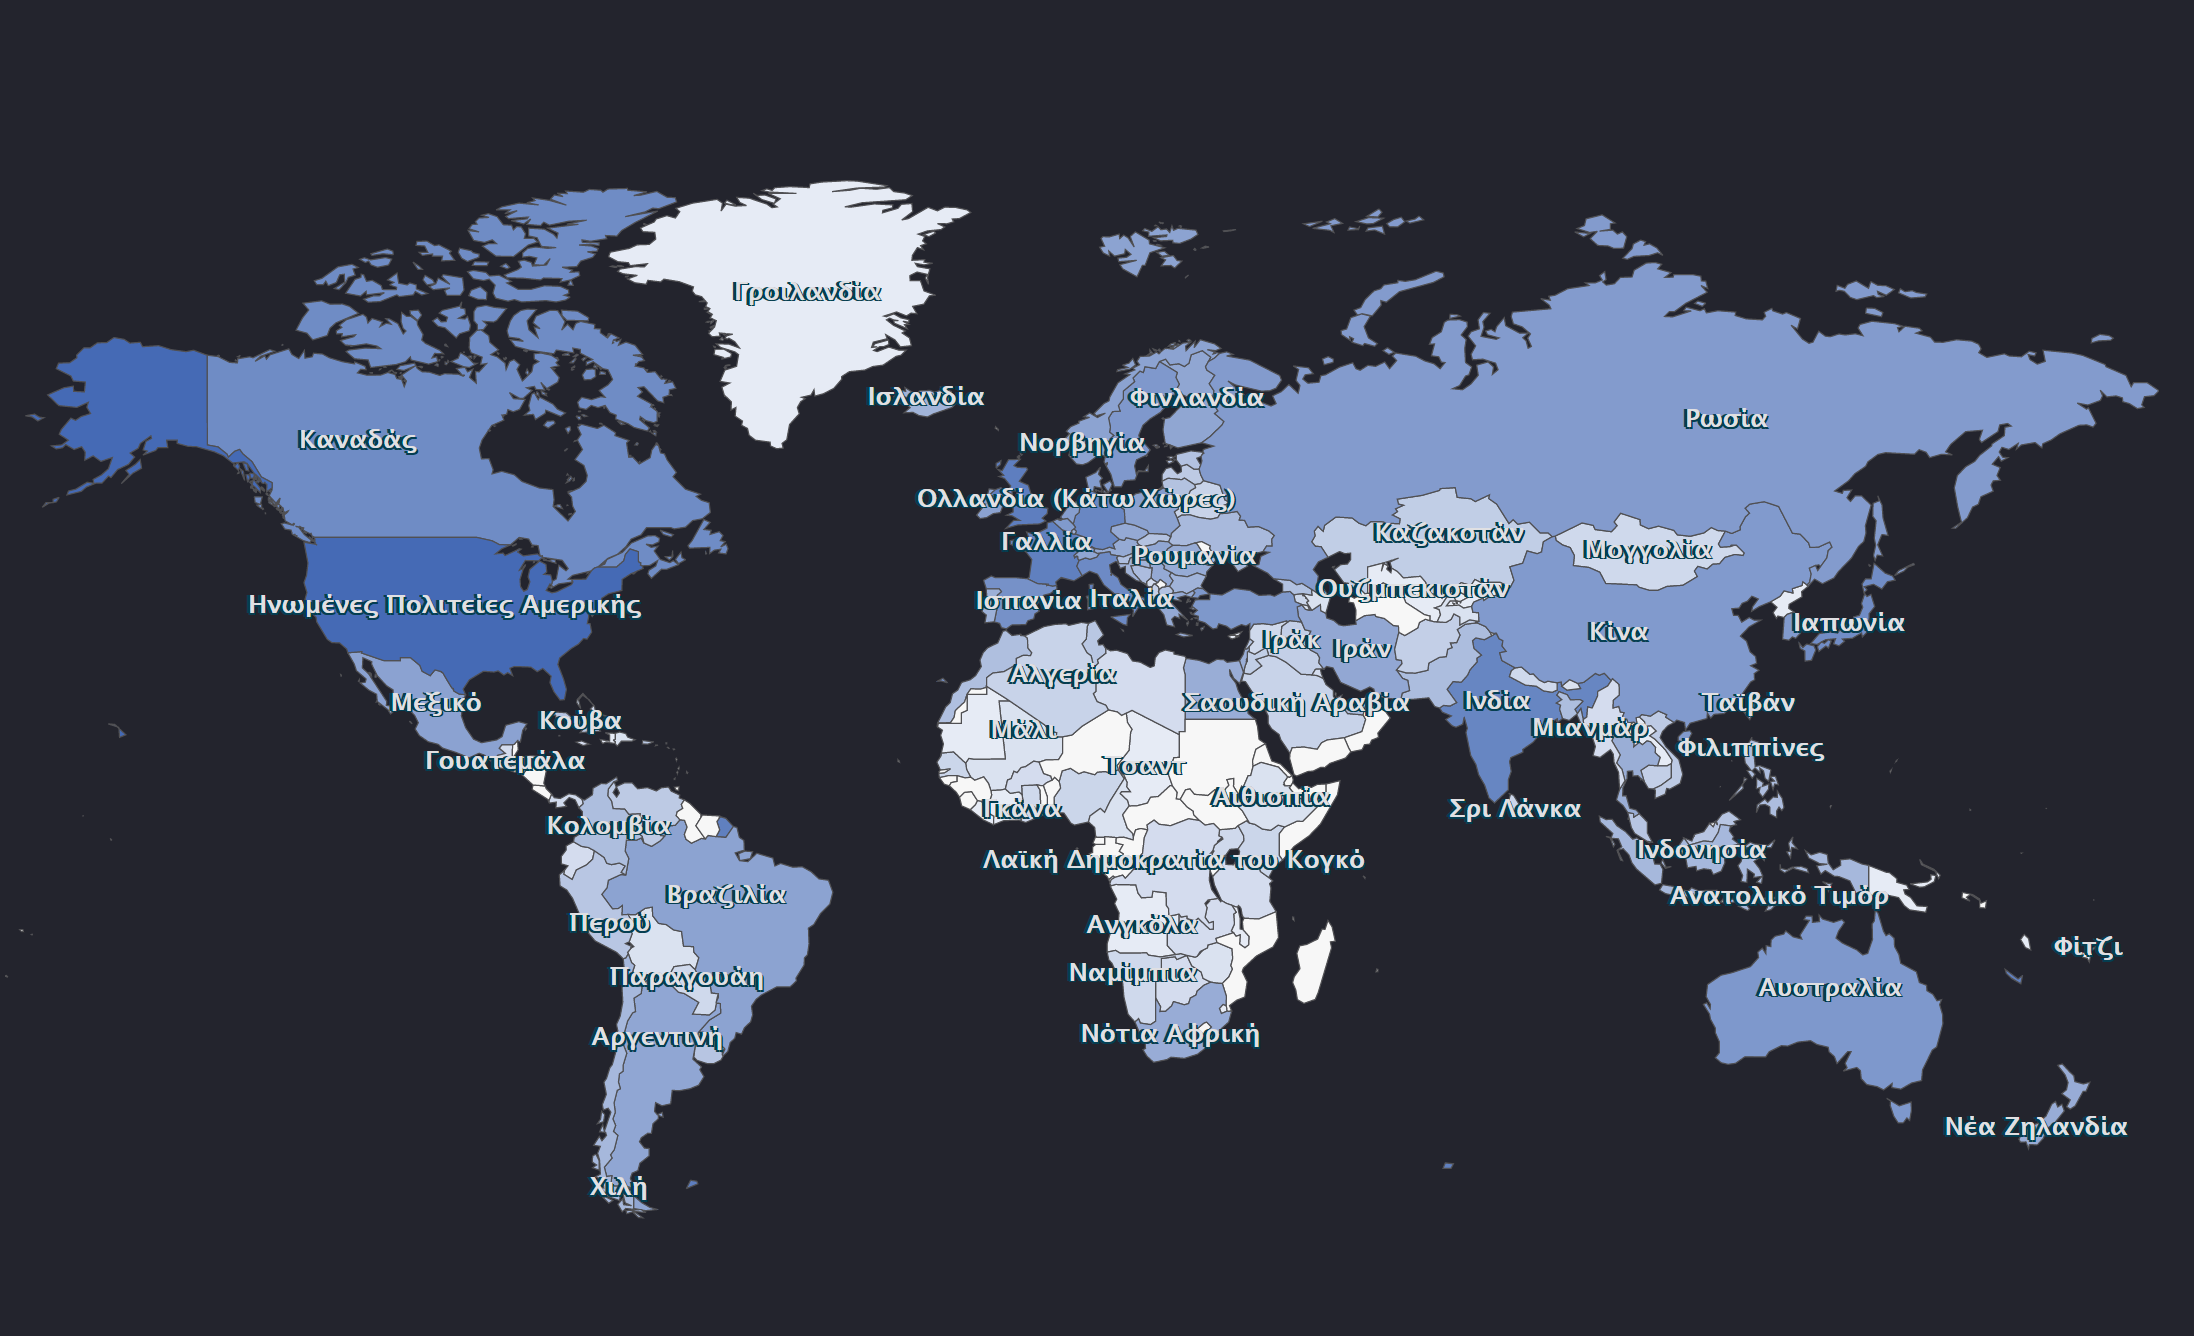
\includegraphics[width=140mm]{Chapters/5 - Architecture/Client/Images/world_map.PNG}
  \caption{Map Component}
  \label{layout:mapcomponent}
\end{figure}

\begin{figure}[H]
    \begin{TypeScriptcode}
countrySelected = (data: ICountryData) => {
  this.props.history.push(AppUtils.|$\textbf{generateNavigationLink}$|({id: data._id, name: data.name, iso31661: data.iso31661, movies: []} as IProductionCountry))
}
countryUnselected = () => {
  this.props.history.push(`/app`)
}
    \end{TypeScriptcode}
    \caption{Αλγόριθμος αλλαγής διεύθυνσης απο το Map Component.}
   \label{code:map_urlchanger}
\end{figure}
\subsubsection{MISidePane Component}
Το ΜΙSidepane Component είναι το τρίτο Component μέσα στο MIDashboard Component και περιέχει το όνομα της κατηγορίας και μια φωτογραφία αν υπάρχει
για παράδειγμα αν είναι η κατηγορία ανά ηθοποιό και ο ηθοποιός ονομαζόταν Νικόλαος Μαυρόπουλος θα εμφάνιζε αυτό το άτομο και την φωτογραφία του αν υπάρχει στην βάση δεδομένων. Περιέχει επίσης ένα Component για την δυνατότητα φιλτραρίσματος των αποτελεσμάτων ανα χρόνο, το MIYearPicker Component, και παρακάτω 4 ίδια Component τύπου MIChartCard για εμφάνιση δεδομένων και γραφημάτων συνδυαστικά. Επί το πλείστον η διάταξη του MISidePane Component παραμένει σταθερή με εξαίρεση την κατηγορία "ανά άτομο" που προστίθεται ένα ακόμα Component το MIRolePicker που δίνει την δυνατότητα φιλτραρίσματος του ρόλου του ατόμου δηλαδή ηθοποιό, σκηνοθέτη, συγγραφέα και παραγωγό.

Το MIChartCard αποτελείται από ένα Grid το οποίο περιέχει ένα γράφημα Highcharts LineChart που στην ουσία είναι ένα γράφημα με μια η περισσότερες γραμμές, ένα εικονίδιο ακριβώς πάνω στο γράφημα περιγραφικό για τι δεδομένα παρουσιάζονται, και δεδομένα από κάτω. Τα δεδομένα του γραφήματος αναπτύσσουν ένα η παραπάνω ποσοτικό πεδίο ανά χρόνο για όσα χρόνια υπάρχουν στην συγκεκριμένη επιλεγμένη κατηγορία, ενώ τα δεδομένα από κάτω εμφανίζουν είτε τα μέγιστα, είτε τα ελάχιστα, είτε τους μέσους όρους των δεδομένων όπως φαίνεται στο σχήμα \ref{layout:michartcard}. Τα γραφήματα των MIChartCard Components όταν φιλτράρεται η κατηγορία ανά χρόνο απενεργοποιούνται, αλλά τα δεδομένα παρακάτω που αναγράφουν μέγιστα ελάχιστα και μέσους όρους παραμένουν και αναφέρονται στο επιλεγμένο έτος για αυτήν την κατηγορία. Δεν υπήρχε ουσιαστικός λόγος τα γραφήματα να έχουν δεδομένα καθώς αυτό που βλέπει ο χρήστης δεν είναι τα συνολικά δεδομένα παρά μόνο του επιλεγμένου έτους.

\begin{figure}[h]
  \centering
  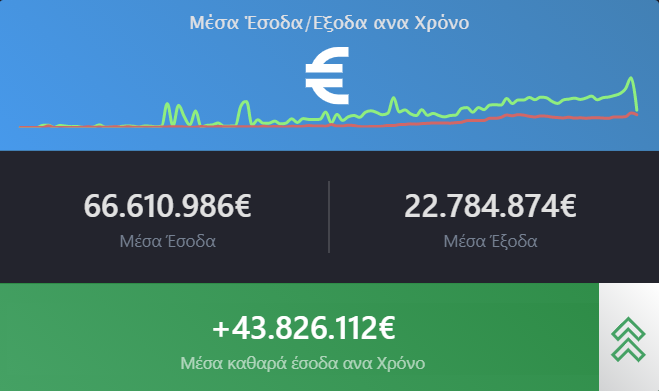
\includegraphics[width=80mm]{Chapters/5 - Architecture/Client/Images/michardcard.png}
  \caption{MIChartCard Component}
  \label{layout:michartcard}
\end{figure}
Το MIYearPicker Component αποτελείται απο 2 κουμπιά και ένα πεδίο εισαγωγής όπως φαίνεται στο σχήμα \ref{layout:miyearpicker}. Όταν πατηθεί το κουμπί με το εικονίδιο ενός ημερολογίου η το πεδίο εισαγωγής, ανοίγει ενα μενού που επιτρέπει την επιλογή ενός έτους που υπάρχει για την επιλεγμένη κατηγορία ενώ οταν πατηθεί το κουμπι με εικονίδιο ενα "Χ" καθαρίζεται η επιλογή του έτους και εμφανίζονται τα συνολικά δεδομένα. Όταν εκτελεστεί μια ενέργεια απο αυτο το Component, θα αλλάξει την διεύθυνση έτσι ώστε να αναλάβει το Dashboard Module την αλλαγή των δεδομένων όπως φαίνεται στον κώδικα \ref{code:miyearpicker_urlchanger}.
\begin{figure}[h]
  \centering
  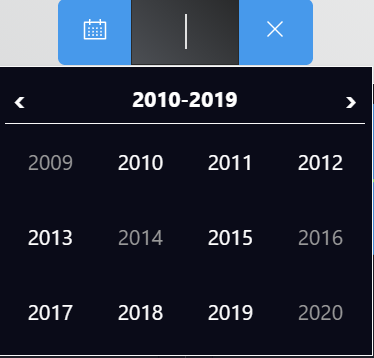
\includegraphics[width=35mm]{Chapters/5 - Architecture/Client/Images/miyearpicker.png}
  \caption{MIYearPicker Component}
  \label{layout:miyearpicker}
\end{figure}

\begin{figure}[h]
    \begin{TypeScriptcode}
yearSelected = (year: number) => {
  const activeView = this.props.rootState.dashboardState.activeView();
  const activeEntity = this.props.rootState.dashboardState.activeView().activeEntity;
  let role = null;
  if (activeView.entityType === EntityType.PERSON) {
    const _activeView = activeView as MovieInsightsPerPersonState;
    role = _activeView.activeRole;
  }
  this.props.history.push(AppUtils.|$\textbf{generateNavigationLink}$|(activeEntity.entity, role, year))
}
yearUnselected = () => {
  const activeEntity = this.props.rootState.dashboardState.activeView().activeEntity;
  if (activeEntity.entity) {
    this.props.history.push(AppUtils.|$\textbf{generateNavigationLink}$|(activeEntity.entity));
  } else {
    this.props.history.push(`/app`);
  }
}
    \end{TypeScriptcode}
    \caption{Αλγόριθμος αλλαγής διεύθυνσης απο το MIYearPicker Component.}
   \label{code:miyearpicker_urlchanger}
\end{figure}
Το MIRolePicker Component εμφανίζεται μόνο όταν η επιλεγμένη κατηγορία είναι "ανά άτομο". Αποτελείται από 4 κουμπιά μονής επιλογής. Αυτό σημαίνει ότι όταν πατηθεί ένα κουμπί επιλέγεται μένει πατημένο και οποιαδήποτε άλλο κουμπί ήταν πατημένο πρωτύτερα αφαιρείται η επιλογή του. Λειτουργεί ακριβώς με τον ίδιο τρόπο με τα παραδοσιακά Radio Buttons. Τα 4 κουμπιά αντιστοιχούν στους 4 ρόλους που μπορεί να έχει ένα άτομο όπως Ηθοποιός, Σκηνοθέτης, Συγγραφέας και Παραγωγός όπως φαίνεται στο σχήμα \ref{layout:mirolepicker}. Όταν ένα Role είναι επιλεγμένο το ανάλογο κουμπί επιλέγεται και εμφανίζεται με χρώμα μπλε, όταν δεν υπάρχει το συγκεκριμένο Role στο άτομο είναι απενεργοποιημένο και εμφανίζεται με χρώμα ανοιχτό γκρι, και αν υπάρχει και δεν είναι επιλεγμένο εμφανίζεται με χρώμα σκούρο γκρι και ο κώδικας επιλογής φαίνεται στο σχήμα. Όταν αλλάζει η επιλογή ο κώδικας που αλλάζει την διεύθυνση φαίνεται στο σχήμα \ref{code:mirolepicker_urlchanger}.
\begin{figure}[h]
  \centering
  
\includegraphics[width=55mm]{Chapters/5 - Architecture/Client/Images/mirolepicker.png}
  \caption{MIRolePicker Component}
  \label{layout:mirolepicker}
\end{figure}

\begin{figure}[H]
    \begin{TypeScriptcode}
private onCreditSelect = (credit: CreditRole) => {
  const activeView = this.props.rootState.dashboardState.activeView() as MovieInsightsPerPersonState;
  this.props.history.push(AppUtils.|$\textbf{generateNavigationLink}$|(activeView._activeEntity.person, credit, activeView.isPerYear ? activeView.activeYearEntity.entity : null));
}
    \end{TypeScriptcode}
    \caption{Αλγόριθμος αλλαγής διεύθυνσης από το MIRolePicker Component.}
   \label{code:mirolepicker_urlchanger}
\end{figure}



\subsubsection{MIInsightsPanel Component}
Το MIInsightsPanel Component είναι το τέταρτο και τελευταίο Component που βρίσκεται μέσα στο MIDashboard Component.
Περιέχει πολλά Component ίδιου τύπου MICard Component. Το κάθε MICard Component είναι μια "κάρτα" που εμφανίζει ένα στοιχείο για ένα άτομο, μια ταινία, μια εταιρία παραγωγής, μια χώρα παραγωγής η ένα είδος ταινίας. Για παράδειγμα αν μια κάρτα για μια ταινία με τα μεγαλύτερα έσοδα θα εμφανιζόταν όπως στο σχήμα \ref{layout:micard_revenue}.

\begin{figure}[h]
  \centering
  
\includegraphics[width=50mm]{Chapters/5 - Architecture/Client/Images/micard_revenue.png}
  \caption{MICard Component}
  \label{layout:micard_revenue}
\end{figure}

Το MICard Component είναι ένα Component το οποιο έχει σχεδιαστεί με ρευστή διάταξη και δυναμικό περιεχόμενο. Ανάλογα με το τι περιεχόμενο θα του δοθεί θα αλλάξει την διάταξη του και θα εμφανίσει τα ανάλογα δεδομένα. Υποστηρίζει Placeholders για την αναμονή των απομακρυσμένων δεδομένων εμφανίζοντας ένα Spinner, και υποστηρίζει και την εμφάνιση ενός μηνύματος λάθους σε περίπτωση που τα δεδομένα για την συγκεκριμένη κατηγορία δεν υπάρχουν. Επιπρόσθετα κάθε Component τυπου MICard μπορεί να πατηθεί σαν κουμπί και ανάλογα με το περιεχόμενο αλλάζει την διεύθυνση στην γραμμή διεύθυνσης του Browser, έτσι ώστε να εμφανιστούν τα ανάλογα δεδομένα μετέπειτα απο το Dashboard Module. Όλα τα MICard λειτουργούν με τον ίδιο τρόπο εκτός απο το MICard που περιέχει δεδομένα ταινιών. Καθώς ο ρόλος της εφαρμογής δεν είναι να εμφανίζει αναλυτικά στοιχεία για ταινίες επειδή υπάρχουν ήδη πολυ γνωστές υπηρεσίες για αυτόν τον σκοπό όπως προαναφέρθηκαν το IMDb και το TMDb, όταν πατηθεί ένα MICard με περιεχόμενο ταινιών θα εμφανιστεί ενα παράθυρο πάνω απο την εφαρμογή το οποίο είναι το MIMovieInfoModal Component όπως φαίνεται στον κώδικα \ref{code:micard_click}.
\begin{figure}[H]
    \begin{TypeScriptcode}
|\textbf{renderCardLinked}|() {
  const link = this.state.entity?AppUtils.|\textbf{generateNavigationLink}|(this.state.entity):''
  return (<NavLink className="mi-card-link" onClick={this.onLinkClick} to={link}>{this.renderCard()}|</NavLink>|);
}
_render() {
  return (
    <>
      {this.state.loaded && this.state.entity ?this.|\textbf{renderCardLinked}|() : this.renderCard()}
      {this.props.entityType === TmdbEntityType.MOVIE ?(|\textbf{<MIMovieInfoModal}| open={this.state.modal} onClose={() => this.setState({modal: false})} entity={this.props.entity as any}|\textbf{/>}|) : null}
    |</>|
  )
}
    \end{TypeScriptcode}
    \caption{Αλγόριθμος αλλαγής διεύθυνσης από το MIRolePicker Component.}
   \label{code:micard_click}
\end{figure}


Το MIMovieInfoModal Component περιέχει το πόστερ της ταινίας καθώς και μια εικόνα background σχετική με την ταινία και περιέχει τα πολύ βασικά στοιχεία που χρησιμοποιεί η εφαρμογή όπως, τα έσοδα, τα έξοδα, την βαθμολογία με της ψήφους της ταινίας καθώς και το πόσο διαρκεί η ταινία συνολικά. Επιπρόσθετα δίνει την επιλογή για περισσότερα στοιχεία για αυτήν την ταινία προσφέροντας 2 συνδέσμους ανακατεύθυνσης που ο ένας πηγαίνει τον χρήστη στον ισότοπο του TMDb στην επιλεγμένη ταινία και ο άλλος στο IMDB όπως φαίνεται στο σχήμα \ref{layout:mimoviemodal}

\begin{figure}[H]
  \centering
  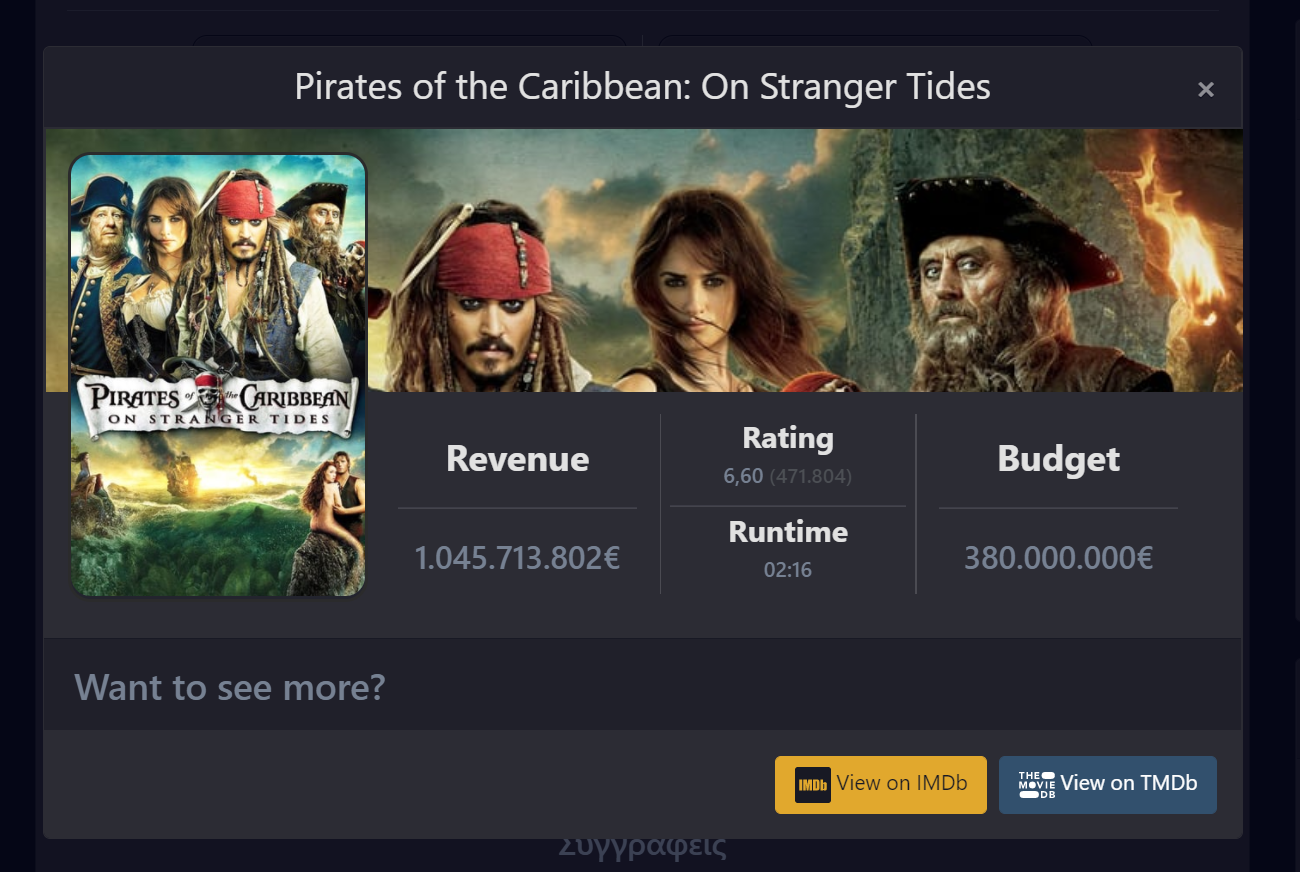
\includegraphics[width=100mm]{Chapters/5 - Architecture/Client/Images/mimoviemodal.png}
  \caption{MIMovieInfoModal Component}
  \label{layout:mimoviemodal}
\end{figure}